\section{Smart Governance}
\label{sec:smart_governance}

%Wie ist der Stand bei Smart Governance in Hamburg?
Um das Ziel der Smart Governance in einer Stadt zu erreichen, sollte sie mit Fokus auf vier grundlegende Dimensionen umgestaltet werden.
\begin{enumerate}
	\item Smarte Regierung
	\item Offene \& verknüpfte Daten
	\item Digitaler Service \& kooperative Regierung
	\item Stadtinfrastruktur
\end{enumerate}
\autocite[14]{Fuetterer.2020}
\\ Quantitativ werden diese Dimensionen bereits durch verschiedene Projekte vorangetrieben. Im Portal \glqq Smart City Kompass\grqq\space werden in ganz Hamburg mehr Smart-Governance-Projekte durchgeführt als in jeder anderen deutschen Stadt \autocite{SmartCityKompass.2020}. Um die Qualität dieser Projekte herauszufinden, wird ein Projekt exemplarisch detailliert untersucht und bewertet.

%Welche Beispielprojekte belegen das?

Im Jahr 2012 verabschiedete die hamburger Regierung ein neuartiges Gesetz, das zu einem Grundpfeiler für die Weiterentwicklung von Open-Government-Initiativen nicht nur in Hamburg sondern auch in vielen anderen Städten Deutschlands werden sollte. Das Ziel des Gesetzes war es, Informationen aus der Senatsarbeit der Allgemeinheit unmittelbar zugänglich zu machen \autocite{Senat.2012}. Die Regelungen in diesem Gesetz wurden umgesetzt mithilfe einer neu entwickelten Online-Plattform, dem \glqq Transparenzportal\grqq.


Diese frei zugängliche Website ermöglicht es jedem Bürger frei über das Internet Daten aus der hamburger Senatsarbeit einzusehen. Abbildung \ref{fig:3_transparenzportal} zeigt beispielhaft die verfügbaren Datensätze, wenn Bürger nach Daten zum Bauprojekt der Elbphilharmonie suchen. Als Ergebnis werden Mitteilungen und Verträge angezeigt, insgesamt sind allein für diesen Suchbegriff über 250 Einträge verfügbar. Interessierte Bürger können so Einsicht in dieses Projekt erhalten um die Arbeit der gewählten Volksvertreter zu kontrollieren und sich transparent eine Meinung zu bilden. Das Portal stellt darüber hinaus auch Verträge, interne Berichte, Haushaltspläne und Weitere Dokumente für die Bürger frei zur Verfügung.

\begin{figure}
	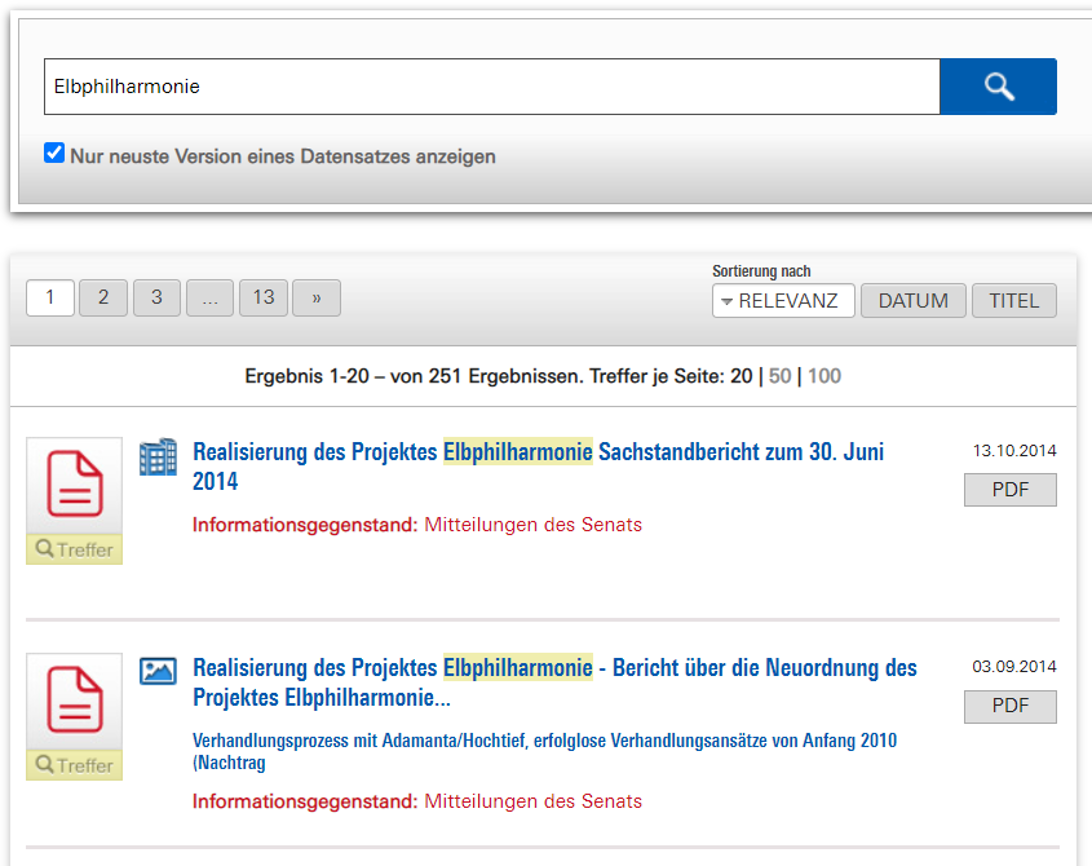
\includegraphics[width=\textwidth]{graphics/3-transparenzportal}
	\caption[Suchergebnisse im Transparenzportal Hamburg]{Suchergebnisse im Transparenzportal Hamburg}
	\label{fig:3_transparenzportal}
\end{figure}

Dieses Projekt bildet für die Stadt Hamburg einen großen Fortschritt im Bereich der digitalen Services sowie der offenen Daten. Die Regierungsdaten sind seitdem offen verfügbar und bilden deswegen, wie in \citeauthor[15]{Fuetterer.2020} beschrieben, einen großen Schritt auf dem Weg zum Open Government. Unterstrichen wird diese Entwicklung durch das Portal transparenzranking.de. Im Vergleich von verschiedenen Transparenzregelungen nimmt Hamburg dort den ersten Platz unter allen deutschen Bundesländern ein.

Das hamburger Transparenzgesetz bringt Fortschritte hauptsächlich in Dimension 2 und 3 der Smart Governance. Die Offenheit der Daten aus Dimension 2 ist komplett erfüllt, fast alle Bürger können Daten der hamburger Regierung schnell, kostenfrei und mit wenig Aufwand einsehen. Außen vor sind nur Bürger ohne Zugang zum Internet, diese Bürger stellen aber nur einen kleinen Anteil der Bevölkerung dar \autocite[10]{Fuetterer.2020}. Aus Dimension 3 ist die Digitalisierung der Services ebenfalls stark verbessert, wobei andere Services des täglichen Lebens in diesem Projekt nicht digitalisiert wurden. 


%Auf welchem Weg ist Hamburg auf dem Weg zur Smart City im Bereich der Smart Governance?



%- Interaktion zwischen Bevölkerung und Regierung soll durch "Open Government Data" befördert werden
%- Definition "Offene Daten"
%  - Verfügbarkeit (in zweckmäßiger Form und zu möglichst niedrigen Kosten)
%  - Wiederverwendung (daten müssen (auch maschinell) verarbeitbar sein)
%  - Universelle Beteiligung (Nutzung jeder Person ermöglicht)
%-  Ziele, um Open Government zu erreichen
%  - Transparenz
%  - Beteiligung
%  - Zusammenarbeit